\documentclass[tikz, border=1mm]{standalone}
\usepackage{helvet}
\renewcommand{\familydefault}{\sfdefault}
\usepackage{tikz}
\usetikzlibrary{calc,patterns,decorations.pathmorphing,decorations.markings,math,intersections,positioning,arrows.meta,graphs,backgrounds,decorations.pathreplacing,calligraphy}
\tikzset{%
between/.style args={#1 and #2}{%
at = ($(#1)!0.5!(#2)$)
},
between base/.style args={#1 and #2}{%
between=#1.base and #2.base
}
}
\usepackage[european, straightvoltages, nooldvoltagedirection]{circuitikz}
\usepackage{bondgraphs}

\begin{document}
%\input{Tikz-Bilder/control.tikzstyles}
\begin{tikzpicture}[node distance=1.5cm]
		% I-Regulator
		\node [integral, label={below:I-Regler}] (I-Reg) at (0,0) {};
		\node [limiter] (I-Lim) [right of=I-Reg] {};
		\node [sum] (sum) [right of=I-Lim] {};
		\node [limiter] (All-Lim) [right of=sum] {};
		\node [pulse, label={[align=center] below:Pulsweiten-\\Modulator}] (PulseModulator) [right of=All-Lim] {};
		% D-Regulator
		\node [differential, label={below:D-Regler}] (D-Reg) [below of=I-Reg] {};
		\node [limiter] (D-Lim) [right of=D-Reg] {};
		% P-Regulator
		\node [proportional, label={below:P-Regler}] (P-Reg) [above of=I-Reg] {};
		\node [limiter] (P-Lim) [right of=P-Reg] {};
		% PP-Regulator
		\node [proportional, label={above:Gain-Regler}] (PP-Reg) [above of=P-Reg] {};
		\node [limiter] (PP-Lim) [right of=PP-Reg] {};
        \node (PP_h) at ($ (sum|-PP-Lim) + (0,-.6) $) {};
        % Input and Knots
		\node [splitter] (knot1) [left of=I-Reg] {};
		\node [splitter] (knot2) [left of=P-Reg] {};
		\node [input] (input) [left of=knot1] {};
        \node (output) [node distance=1.5cm, right of=PulseModulator]{};
        
        %% Edges
        \draw [signal] (input) -- (knot1) -- (I-Reg);
        % I-Regulator
        \draw [signal] (I-Reg) -- (I-Lim);
        \draw [signal] (I-Lim) -- (sum) node [xshift=-0.6cm, above] {\footnotesize$+$};
        % D-Regulator
		\draw [signal] (knot1) |- (D-Reg);
		\draw [signal] (D-Reg) -- (D-Lim);
		\draw [signal] (D-Lim) -| (sum) node [yshift=-0.6cm, left] {\footnotesize$+$};
		% P-Regulator
		\draw [signal] (knot1) |- (P-Reg);
		\draw [signal] (P-Reg) -- (P-Lim);
		\draw [signal] (P-Lim) -| (sum) node [yshift=0.6cm, right] {\footnotesize$+$};
		% PP-Regulator
		\draw [signal] (knot1) |- (PP-Reg);
		\draw [signal] (PP-Reg) -- (PP-Lim);
		\draw [signal] (PP-Lim) -| (PP_h.center) -| (P-Reg);
		% Output
		\draw [signal] (sum) -- (All-Lim);
		\draw [signal] (All-Lim) -- (PulseModulator);
		\draw [signal] (PulseModulator) -- (output);
\end{tikzpicture}
\input{Tikz-Bilder/control.tikzstyles}
\begin{tikzpicture}[
    node distance=1cm
    ]
    % Asynchronmaschine
    \node (Netz_in) [bgelement] {Netz-Eingang};
    \node (ASM_Stator) [bgelement, below=of Netz_in] {Stator};
    %\node (ASM_Stator_R) [bgelement, above left=of ASM_Stator] {R};
    %\node (ASM_Stator_L) [bgelement, below left=of ASM_Stator] {L};
    \node (ASM_Luftspalt) [bgelement, below=of ASM_Stator] {Luftspalt};
    \node (ASM_Rotor) [bgelement, below=3cm of ASM_Luftspalt] {Rotor};
    %\node (ASM_Rotor_R) [bgelement, above left=of ASM_Rotor] {R};
    %\node (ASM_Rotor_L) [bgelement, below left=of ASM_Rotor] {L};
    \draw[bonds]
    (Netz_in) edge[flow=$i_{\mathrm{ein}}$, effort=$u_{\mathrm{ein}}$] (ASM_Stator)
    (ASM_Stator) %edge (ASM_Stator_R)
                 %edge (ASM_Stator_L)
                 edge[flow=$\Phi_{\mathrm{s}}$, effort=$V_{\mathrm{m,s}}$] (ASM_Luftspalt)
    (ASM_Luftspalt) edge[flow=$\Phi_{\mathrm{r}}$, effort=$V_{\mathrm{m,r}}$] (ASM_Rotor);
    %(ASM_Rotor) edge (ASM_Rotor_R)
    %            edge (ASM_Rotor_L);
    
    % Mechanik
    \node (Welle) [bgelement, right=1.1cm of ASM_Rotor] {Welle};
    % \node (Reibung) [bgelement, below =of Welle] {Reibung};
    
    \node (Gleichrichter) [bgelement, right=1cm of Welle] {Gleichrichter};
    \draw[bonds] 
        (ASM_Rotor) edge[effort=$M_{\mathrm{Motor}}$, flow=$\omega$] (Welle);
        % (Welle) edge[effort=$M_{\mathrm{Verl.}}$, flow=$\omega$] (Reibung);
    
     % Synchro-Generator
    \node (SG_Luftspalt) [bgelement] at (Gleichrichter|-ASM_Luftspalt.base) {Luftspalt};
    \node (SG_Rotor_Y) [between= Gleichrichter and SG_Luftspalt] {};
    \node (SG_Rotor) [bgelement] at (Gleichrichter|-SG_Rotor_Y) {Rotor};
    %\node (SG_Rotor_R) [bgelement, above right=of SG_Rotor] {R};
    %\node (SG_Rotor_L) [bgelement, below right=of SG_Rotor] {L};
    \node (SG_Stator) [bgelement] at (SG_Luftspalt|-ASM_Stator.base) {Stator};
    %\node (SG_Stator_R) [bgelement, above right=of SG_Stator] {R};
    %\node (SG_Stator_L) [bgelement, above left=of SG_Stator] {L};
    \draw[bonds]
    (Welle) edge[effort=$M_{\mathrm{Gen.}}$, flow=$\omega$] (SG_Rotor)
    (Gleichrichter) edge[effort=$u_{\mathrm{DC}}$, flow=$i_{\mathrm{DC}}$] (SG_Rotor)
    (SG_Rotor) edge[flow=$\Phi_{\mathrm{r}}$, effort=$V_{\mathrm{m,r}}$] (SG_Luftspalt)
               %edge (SG_Rotor_R)
               %edge (SG_Rotor_L)
    (SG_Luftspalt) edge[flow=$\Phi_{\mathrm{s}}$, effort=$V_{\mathrm{m,s}}$] (SG_Stator);
    %(SG_Stator) edge (SG_Stator_R)
    %            edge (SG_Stator_L);
    
    % Erregermaschine
    \node (EM_Rotor) [bgelement, below=of Gleichrichter] {Rotor};
    %\node (EM_Rotor_R) [bgelement, below left=of EM_Rotor] {R};
    %\node (EM_Rotor_L) [bgelement, below right=of EM_Rotor] {L};
    \node (EM_Luftspalt) [bgelement, right=of EM_Rotor] {Luftspalt};
    \node (EM_Stator) [bgelement, right=of EM_Luftspalt] {Stator};
    %\node (EM_Stator_R) [bgelement, below left=of EM_Stator] {R};
    %\node (EM_Stator_L) [bgelement, below right=of EM_Stator] {L};
    
    \draw[bonds]
    (Welle) edge[effort=$M_{\mathrm{Err.}}$, flow=$\omega$] (EM_Rotor)
    (EM_Rotor) edge[effort=$u_{\mathrm{AC}}$, flow=$i_{\mathrm{AC}}$] (Gleichrichter)
               %edge (EM_Rotor_L)
               %edge (EM_Rotor_R)
    (EM_Luftspalt) edge[flow=$\Phi_{\mathrm{r}}$, effort=$V_{\mathrm{m,r}}$] (EM_Rotor)
    (EM_Stator) edge[flow=$\Phi_{\mathrm{s}}$, effort=$V_{\mathrm{m,s}}$] (EM_Luftspalt);
                %edge (EM_Stator_R)
                %edge (EM_Stator_L);
    
    % Last
    \node (Last) [bgelement] at (EM_Stator|-SG_Stator) {Last};
    \draw[bonds] (SG_Stator) edge[flow=$i_{\mathrm{aus}}$, effort=$u_{\mathrm{aus}}$] (Last);
    
    % Regler
    \node (Summe) [sum, below=of Last] {};
    \node (Sollspannung) [input, right=of Summe, label=$U_{\mathrm{aus,soll}}$] {};
    \node (Regler) [block, label={right:}] at ($(Summe)!1/3!(EM_Stator)$) {PID};
    \node (PWM) [pulse, label={right:PWM}] at ($(Summe)!2/3!(EM_Stator)$) {};
    \draw[signal] (Last) -- node[left] (U_Regler_in) {$U_{\mathrm{aus,ist}}$} (Summe);
    \draw[signal] (Sollspannung) -- node[near end,below]{\small $-$} (Summe);
    \draw[signal] (Summe) -- (Regler);
    \draw[signal] (Regler) -- (PWM);
    \draw[bonds] (PWM) ++(0,-.6) edge[effort=$u_{\mathrm{err}}$, flow=$i_{\mathrm{err}}$] (EM_Stator);
    
    %Beschriftung
    \node [below=.3cm of EM_Luftspalt] {Erregermaschine};
    \node [above=.3cm of SG_Stator] {Synchrongenerator};
    \node [below=.3cm of ASM_Rotor] {Asynchronmaschine};
    \node [right=.3cm of Regler, align=center] {Regler-\\ board};
    \begin{pgfonlayer}{background}
    \filldraw [line width=4mm,join=round,black!5]
      (Netz_in.west|-Netz_in.north)  rectangle (Netz_in.east|-ASM_Rotor.south)
      (SG_Luftspalt.west|-SG_Stator.north) rectangle (SG_Luftspalt.east|-SG_Rotor.south)
      ($(EM_Rotor.west|-EM_Rotor.north) + (0,.1)$) rectangle ($(EM_Stator.east|-EM_Stator.south) + (0,-.1)$);
      %($(U_Regler_in.west) + (0,.2)$) rectangle ($(Sollspannung.east|-PWM.east) + (.4,-.4)$);
  \end{pgfonlayer}
\end{tikzpicture}
%\input{Tikz-Bilder/control.tikzstyles}
\tikzstyle{load jump}=[block, path picture={
    % Axes
    \node[block axes]{};
    % Plot function
    \draw[thick] plot[smooth] coordinates {%
    (-.4,.2) (-.3,.2) (-.2,.2) (-.18,-.1) (-.16,-.1) (-.08,.2) (0,.2) (.45,.2)
    };
}]
\tikzstyle{ises}=[block, path picture={
    % Axes
    \node[block axes]{};
    % Plot function
    \draw[thick] plot[smooth] coordinates {%
    (-.3,.2) (-.1,-.15) (.3,-.22) 
    };
    %\draw[thick] plot[smooth] coordinates {%
    %(-.3,-.3) (-.1,-.28) (.3,-.05) 
    %};
}]
\tikzstyle{trends}=[block, path picture={
    % Axes
    \draw[thick] ++(-0.4,-0.3) +(0,.6) |- +(.3,0) ++(.5,0) +(0,.6) |- +(.3,0);
    % Plot function
    \draw[mark=x, only marks, mark size=1pt] plot coordinates {
        % Left side
        (-.25,-.25)
        (-.3,-.15)
        (-.2,-.15)
        (-.25,-.05)
        (-.25,.05)
        % Right side
        (.25, -.15)
        (.2, -.1)
        (.3, -.1)
        (.25, 0)
        (.25, .2)
    };
}]

\begin{tikzpicture}[node distance=2cm]
% Nodes
    \node [input, label={left:Daten}] (input) at (0,0) {};
    \node [wide block] (formula) [right of=input] {Umrechnung};
    \node [knot] (knot1) [right of=formula] {};
    
    \node [wide block] (model) [node distance=2cm, right of=knot1] {Modell};
    \node [wide block] (measurement) [below of=model] {Messung};
    
    \node [] (sweeps) [node distance=3cm, right of=model] {};
    \node [load jump, yshift=.1cm, xshift=.1cm] (sweep1) at (sweeps) {};
    \node [load jump] (sweep2) at (sweeps) {};
    \node [load jump, yshift=-.1cm, xshift=-.1cm] (sweep3) at (sweeps) {};
    \node [between=model.east and sweep3.west] (model_sweep) {};
    
    \node [] (ises) [right of=sweeps] {};
    \node [ises, yshift=.1cm, xshift=.1cm] (ise1) at (ises) {};
    \node [ises] (ise2) at (ises) {};
    \node [ises, yshift=-.1cm, xshift=-.1cm] (ise3) at (ises) {};
    
    \node [trends] (trends) [right of=ises] {};

%% Brace + Decoration
    \draw [thick, decorate, decoration = {brace, raise=25pt, amplitude=5pt, mirror}] (sweep3.west |- sweeps.west) -- (trends.east) node[pos=0.5,above=-50pt] {Auswertung};
    
%% Edges
    \draw [signal] (input) -- (formula) -- (knot1);
    \draw [signal] (knot1) -- (model);
    \draw [signal] (measurement) -| (knot1);
    \draw [signal] (model) -- (sweep3.west|-sweeps);
    \draw [signal] (sweep1.east|-sweeps) -- (ise3.west|-ises);
    \draw [signal] (ise1.east|-ises) -- (trends);
    \draw [signal] (model_sweep|-sweeps) |- (measurement);

\end{tikzpicture}
%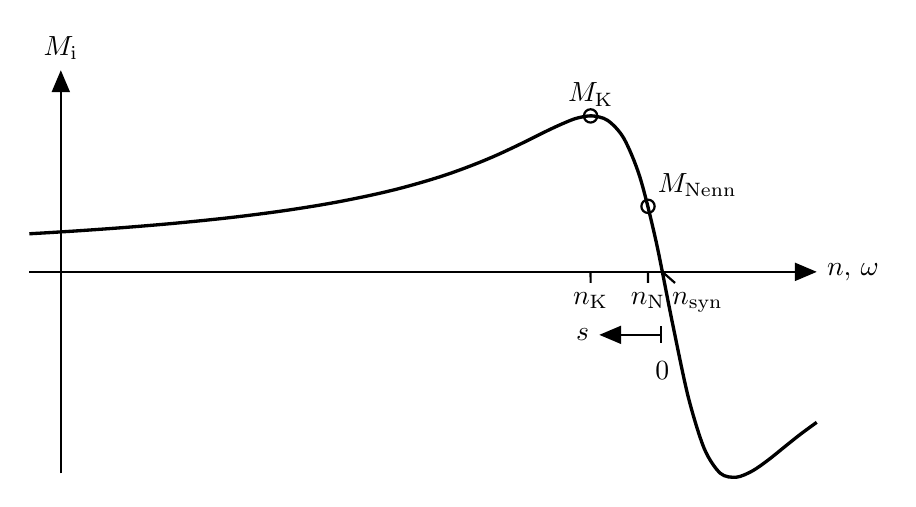
\begin{tikzpicture}[scale=0.8]
\tikzmath{
    \p = 1;
    \ASMms = 3;
    \Us = 100;
    \ASMsigma = 0.067;
    \Xs = 3;
    \Xr = \Xs;
    \Rr = 0.008*\Xr;
    \Rs = 0.01*\Xs;
    \ASMfs = 50;
    \nsyn = 60/2/pi*\ASMfs/\p / (600/12);
    function drehzahl(\s) {
        return (1 - \s)*\ASMfs*60/\p/2/pi;
    };
    \nk = drehzahl(\Rr/\ASMsigma/\Xr) / (600/12);
    \nn = \nk + 0.8*(\nsyn-\nk);
    function schlupf(\n) {
        return 1 - \n*\p/\ASMfs*2*pi/60;  
    };
    function drehmoment(\n) {
        return \ASMms * \p/(2*pi*\ASMfs) * \Us^2 * schlupf(\n)*(1-\ASMsigma)*\Xs*\Xr*\Rr / ((\Rs*\Rr - schlupf(\n)*\ASMsigma*\Xs*\Xr)^2 + (schlupf(\n)*\Rs*\Xr + \Xs*\Rr)^2);
    };
    \Mk = drehmoment(\nk*(600/12))/(250/3.2);
    \Mn = drehmoment(\nn*(600/12))/(250/3.2);
}

    \draw[->, thick, >=triangle 45] (-.5, 0) -- (12, 0) node[right] {$n,\, \omega$};
    \draw[->, thick, >=triangle 45] (0, -3.2) -- (0, 3.2) node[above] {$M_{\mathrm{i}}$};
    
    \node[below right, yshift=-4pt] (nsyn) at (\nsyn, 0) {$n_{\mathrm{syn}}$};
    \node[below, yshift=-4pt] (nk) at (\nk, 0) {$n_{\mathrm{K}}$};
    \node[below, yshift=-4pt] (nn) at (\nn, 0) {$n_{\mathrm{N}}$};
    \node[above] (Mk) at (\nk, \Mk) {$M_{\mathrm{K}}$};
    \node[above right] (Mn) at (\nn, \Mn) {$M_{\mathrm{Nenn}}$};
 
    \draw[thick] (nsyn) -- (\nsyn, 0);
    \draw[thick] (nk) -- (\nk, 0);
    \draw[thick] (nn) -- (\nn, 0);
    \draw[thick] (Mk) -- (\nk, \Mk);
    \draw[thick] (Mn) -- (\nn, \Mn);
    \draw[|->, thick, >=triangle 45] (\nsyn,0) ++(0,-1) node[below, yshift=-6pt] {$0$} -- ++(-1,0) node[left] {$s$}; 
    \draw[mark=*, fill=white, mark options={thick}, only marks, mark size=3pt] plot coordinates {
        (\nk, \Mk) %Kippmoment
        (\nn, \Mn) %Nennmoment
    };
    
    \draw[domain=-.5:12, smooth, variable=\n, very thick, samples=50] plot ({\n}, {drehmoment(\n*(600/12))/(250/3.2)});
\end{tikzpicture}
%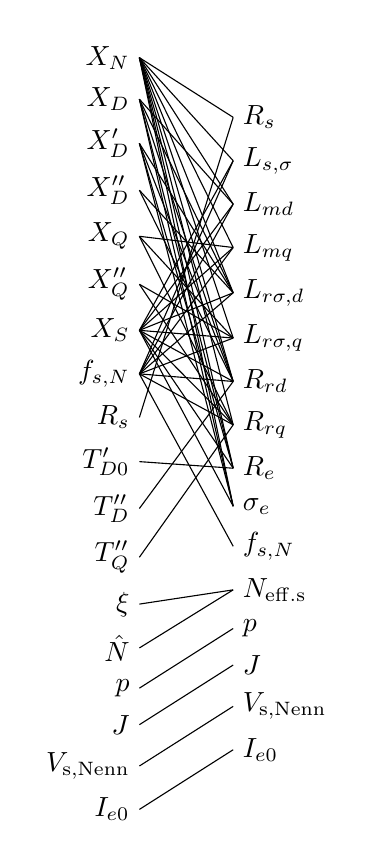
\begin{tikzpicture}[node distance=.5cm]
    % Linke Seite
    \begin{scope}[]
    	    \matrix[column 1/.style={anchor=base east}]{
             \node[] (XN) {$X_N$}; \\
             \node[] (XD) {$X_D$}; \\
             \node[] (XD') {$X_D'$}; \\
             \node[] (XD'') {$X_D''$}; \\
             \node[] (XQ) {$X_Q$}; \\
             \node[] (XQ'') {$X_Q''$}; \\
             \node[] (XS) {$X_S$}; \\
             \node[] (fsNl) {$f_{s,N}$}; \\
             \node[] (Rsl) {$R_s$}; \\
             \node[] (TD0') {$T_{D0}'$}; \\
             \node[] (TD'') {$T_D''$}; \\
             \node[] (TQ'') {$T_Q''$}; \\
             \node[] (xi) {$\xi$};\\
             \node[] (N) {$\hat N$};\\
             \node[] (pl) {$p$};\\
             \node[] (Jl) {$J$};\\             
             \node[] (VsNennl) {$V_{\mathrm{s,Nenn}}$};\\
             \node[] (Ie0l) {$I_{e0}$};\\
        };
    \end{scope}
    % Rechte Seite
    \begin{scope}[xshift=2.5cm]
    	    \matrix[column 1/.style={anchor=base west}]{
             \node[] (Rs) {$R_s$}; \\
             \node[] (Lssigma) {$L_{s,\sigma}$}; \\
             \node[] (Lmd) {$L_{md}$}; \\
             \node[] (Lmq) {$L_{mq}$}; \\
             \node[] (Lrsigmad) {$L_{r\sigma,d}$}; \\
             \node[] (Lrsigmaq) {$L_{r\sigma,q}$}; \\
             \node[] (Rrd) {$R_{rd}$}; \\
             \node[] (Rrq) {$R_{rq}$}; \\
             \node[] (Re) {$R_e$}; \\
             \node[] (sigmae) {$\sigma_e$};\\
             \node[] (fsN) {$f_{s,N}$}; \\
             \node[] (Neff) {$N_{\mathrm{eff.s}}$};\\
             \node[] (p) {$p$};\\
             \node[] (J) {$J$};\\
             \node[] (VsNenn) {$V_{\mathrm{s,Nenn}}$};\\
             \node[] (Ie0) {$I_{e0}$};\\
        };
    \end{scope}
    \draw (XN.east) edge (Rs.west)
               edge (Lssigma.west)
               edge (Lmd.west)
               edge (Lmq.west)
               edge (Lrsigmad.west)
               edge (Lrsigmaq.west)
               edge (Rrd.west)
               edge (Rrq.west)
               edge (Re.west)
               edge (sigmae.west);

    \draw (XD.east) edge (Lmd.west)
               edge (Lrsigmad.west)
               edge (Rrd.west)
               edge (Re.west)
               edge (sigmae.west);
               
    \draw (XD'.east) edge (Lrsigmad.west)
                edge (Rrd.west)
                edge (Re.west)
               edge (sigmae.west);
                
    \draw (XD''.east) edge (Lrsigmad.west)
                 edge (Rrd.west);
                 
    \draw (XQ.east) edge (Lmq.west)
               edge (Lrsigmaq.west)
               edge (Rrq.west);
               
    \draw (XQ''.east) edge (Lrsigmaq.west)
                 edge (Rrq.west);
                 
    \draw (XS.east) edge (Lssigma.west)
               edge (Lmd.west)
               edge (Lmq.west)
               edge (Lrsigmad.west)
               edge (Lrsigmaq.west)
               edge (Rrd.west)
               edge (Rrq.west)
               edge (Re.west)
               edge (sigmae.west);
               
    \draw (fsNl.east) edge (Lssigma.west)
                edge (Lmd.west)
                edge (Lmq.west)
                edge (Lrsigmad.west)
                edge (Lrsigmaq.west)
                edge (Rrd.west)
                edge (Rrq.west)
                edge (fsN.west);
                
    \draw (Rsl.east) edge (Rs.west);
    
    \draw (TD0'.east) edge (Re.west);
    
    \draw (TD''.east) edge (Rrd.west);
    
    \draw (TQ''.east) edge (Rrq.west);
    
    \draw (xi.east) edge (Neff.west);
    
    \draw (N.east) edge (Neff.west);

    \draw (pl.east) edge (p.west);
    
    \draw (Jl.east) edge (J.west);
    
    \draw (VsNennl.east) edge (VsNenn.west);
    
    \draw (Ie0l.east) edge (Ie0.west);    
\end{tikzpicture}

%             \node[] (XN) {$X_N$}; \\
%             \node[below=of XN] (XD) {$X_D$}; \\
%             \node[below=of XD] (XD') {$X_D'$}; \\
%             \node[below=of XD'] (XD'') {$X_D''$}; \\
%             \node[below=of XD''] (XQ) {$X_Q$}; \\
%             \node[below=of XQ] (XQ'') {$X_Q''$}; \\
%             \node[below=of XQ''] (XS) {$X_S$}; \\
%             \node[below=of XS] (fsN) {$f_{s,N}$}; \\
%             \node[below=of fsN] (Rs) {$R_s$}; \\
%             \node[below=of Rs] (TD0') {$T_{D0}'$}; \\
%             \node[below=of TD0'] (TD'') {$T_D''$}; \\
%             \node[below=of TD''] (TQ'') {$T_Q''$}; \\
%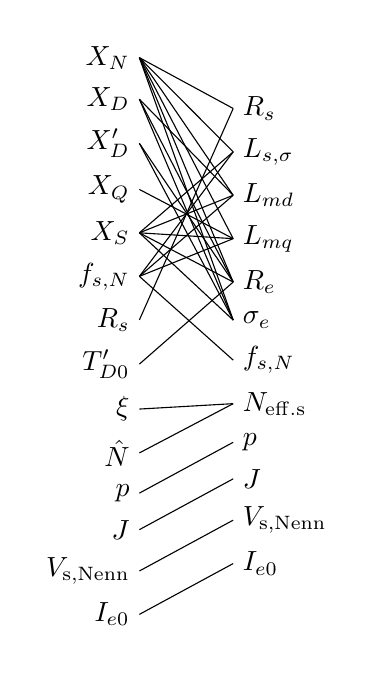
\begin{tikzpicture}[node distance=.5cm]
    % Linke Seite
    \begin{scope}[]
    	    \matrix[column 1/.style={anchor=base east}]{
             \node[] (XN) {$X_N$}; \\
             \node[] (XD) {$X_D$}; \\
             \node[] (XD') {$X_D'$}; \\
             \node[] (XQ) {$X_Q$}; \\
             \node[] (XS) {$X_S$}; \\
             \node[] (fsNl) {$f_{s,N}$}; \\
             \node[] (Rsl) {$R_s$}; \\
             \node[] (TD0') {$T_{D0}'$}; \\
             \node[] (xi) {$\xi$};\\
             \node[] (N) {$\hat N$};\\
             \node[] (pl) {$p$};\\
             \node[] (Jl) {$J$};\\             
             \node[] (VsNennl) {$V_{\mathrm{s,Nenn}}$};\\
             \node[] (Ie0l) {$I_{e0}$};\\
        };
    \end{scope}
    % Rechte Seite
    \begin{scope}[xshift=2.5cm]
    	    \matrix[column 1/.style={anchor=base west}]{
             \node[] (Rs) {$R_s$}; \\
             \node[] (Lssigma) {$L_{s,\sigma}$}; \\
             \node[] (Lmd) {$L_{md}$}; \\
             \node[] (Lmq) {$L_{mq}$}; \\
             \node[] (Re) {$R_e$}; \\
             \node[] (sigmae) {$\sigma_e$};\\
             \node[] (fsN) {$f_{s,N}$}; \\
             \node[] (Neff) {$N_{\mathrm{eff.s}}$};\\
             \node[] (p) {$p$};\\
             \node[] (J) {$J$};\\
             \node[] (VsNenn) {$V_{\mathrm{s,Nenn}}$};\\
             \node[] (Ie0) {$I_{e0}$};\\
        };
    \end{scope}
    \draw (XN.east) edge (Rs.west)
               edge (Lssigma.west)
               edge (Lmd.west)
               edge (Lmq.west)
               edge (Re.west)
               edge (sigmae.west);

    \draw (XD.east) edge (Lmd.west)
               edge (Re.west)
               edge (sigmae.west);
               
    \draw (XD'.east) %edge (Lrsigmad)
                edge (Re.west)
                edge (sigmae.west);
                 
    \draw (XQ.east) edge (Lmq.west);

    \draw (XS.east) edge (Lssigma.west)
               edge (Lmd.west)
               edge (Lmq.west)
               edge (Re.west)
               edge (sigmae.west);
               
    \draw (fsNl.east) edge (Lssigma.west)
                edge (Lmd.west)
                edge (Lmq.west)
                edge (fsN.west);
                
    \draw (Rsl.east) edge (Rs.west);
    
    \draw (TD0'.east) edge (Re.west);
    
    \draw (xi.east) edge (Neff.west);
    
    \draw (N.east) edge (Neff.west);
    
    \draw (pl.east) edge (p.west);
    
    \draw (Jl.east) edge (J.west);
    
    \draw (VsNennl.east) edge (VsNenn.west);
    
    \draw (Ie0l.east) edge (Ie0.west);
\end{tikzpicture}

%             \node[] (XN) {$X_N$}; \\
%             \node[below=of XN] (XD) {$X_D$}; \\
%             \node[below=of XD] (XD') {$X_D'$}; \\
%             \node[below=of XD'] (XD'') {$X_D''$}; \\
%             \node[below=of XD''] (XQ) {$X_Q$}; \\
%             \node[below=of XQ] (XQ'') {$X_Q''$}; \\
%             \node[below=of XQ''] (XS) {$X_S$}; \\
%             \node[below=of XS] (fsN) {$f_{s,N}$}; \\
%             \node[below=of fsN] (Rs) {$R_s$}; \\
%             \node[below=of Rs] (TD0') {$T_{D0}'$}; \\
%             \node[below=of TD0'] (TD'') {$T_D''$}; \\
%             \node[below=of TD''] (TQ'') {$T_Q''$}; \\
%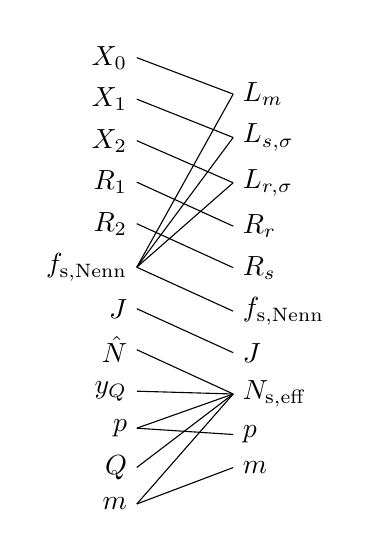
\begin{tikzpicture}[node distance=.5cm]
    % Linke Seite
    \begin{scope}[]
    	    \matrix[column 1/.style={anchor=base east}]{
             \node[] (X0) {$X_0$}; \\
             \node[] (X1) {$X_1$}; \\
             \node[] (X2) {$X_2$}; \\
             \node[] (R1) {$R_1$}; \\
             \node[] (R2) {$R_2$}; \\
             \node[] (fsNennl) {$f_{\mathrm{s,Nenn}}$};\\
             \node[] (Jl) {$J$};\\
             \node[] (N) {$\hat N$};\\
             \node[] (yQ) {$y_Q$};\\
             \node[] (pl) {$p$};\\
             \node[] (Q) {$Q$};\\
             \node[] (ml) {$m$};\\
        };
    \end{scope}
    % Rechte Seite
    \begin{scope}[xshift=2.5cm]
    	    \matrix[column 1/.style={anchor=base west}]{
             \node[] (Lm) {$L_m$}; \\
             \node[] (Lssigma) {$L_{s,\sigma}$};\\
             \node[] (Lrsigma) {$L_{r,\sigma}$};\\
             \node[] (Rr) {$R_r$};\\
             \node[] (Rs) {$R_s$};\\
             \node[] (fsNenn) {$f_{\mathrm{s,Nenn}}$};\\
             \node[] (J) {$J$};\\
             \node[] (Neff) {$N_{\mathrm{s,eff}}$};\\
             \node[] (p) {$p$};\\
             \node[] (m) {$m$};\\
        };
    \end{scope}
    \draw (Lm.west) edge (X0.east)
                    edge (fsNennl.east);

    \draw (Lssigma.west) edge (X1.east)
                    edge (fsNennl.east);

    \draw (Lrsigma.west) edge (X2.east)
                    edge (fsNennl.east);

    \draw (Neff.west) edge (N.east)
                      edge (pl.east)
                      edge (Q.east)
                      edge (ml.east)
                      edge (yQ.east);

    \draw (Rr.west) edge (R1.east);

    \draw (Rs.west) edge (R2.east);

    \draw (fsNenn.west) edge (fsNennl.east);

    \draw (p.west) edge (pl.east);

    \draw (m.west) edge (ml.east);

    \draw (J.west) edge (Jl.east);
\end{tikzpicture}

%             \node[] (XN) {$X_N$}; \\
%             \node[below=of XN] (XD) {$X_D$}; \\
%             \node[below=of XD] (XD') {$X_D'$}; \\
%             \node[below=of XD'] (XD'') {$X_D''$}; \\
%             \node[below=of XD''] (XQ) {$X_Q$}; \\
%             \node[below=of XQ] (XQ'') {$X_Q''$}; \\
%             \node[below=of XQ''] (XS) {$X_S$}; \\
%             \node[below=of XS] (fsN) {$f_{s,N}$}; \\
%             \node[below=of fsN] (Rs) {$R_s$}; \\
%             \node[below=of Rs] (TD0') {$T_{D0}'$}; \\
%             \node[below=of TD0'] (TD'') {$T_D''$}; \\
%             \node[below=of TD''] (TQ'') {$T_Q''$}; \\
%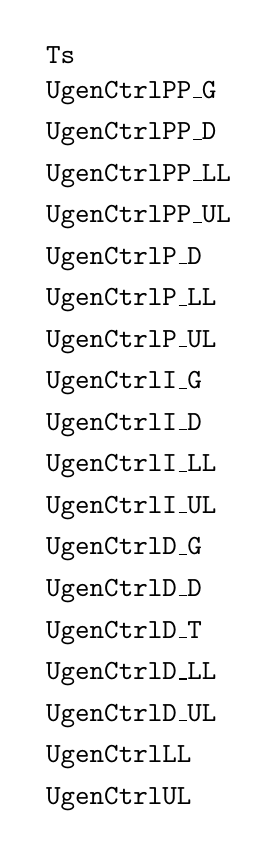
\begin{tikzpicture}[node distance=.5cm]
    \begin{scope}[]
    	    \matrix[column 1/.style={anchor=base west}]{
             \node[] {\texttt{Ts}}; \\
             \node[] {\texttt{UgenCtrlPP\_G}}; \\
             \node[] {\texttt{UgenCtrlPP\_D}}; \\
             \node[] {\texttt{UgenCtrlPP\_LL}}; \\
             \node[] {\texttt{UgenCtrlPP\_UL}}; \\
             \node[] {\texttt{UgenCtrlP\_D}}; \\
             \node[] {\texttt{UgenCtrlP\_LL}}; \\
             \node[] {\texttt{UgenCtrlP\_UL}}; \\
             \node[] {\texttt{UgenCtrlI\_G}}; \\
             \node[] {\texttt{UgenCtrlI\_D}}; \\
             \node[] {\texttt{UgenCtrlI\_LL}}; \\
             \node[] {\texttt{UgenCtrlI\_UL}}; \\
             \node[] {\texttt{UgenCtrlD\_G}}; \\
             \node[] {\texttt{UgenCtrlD\_D}}; \\
             \node[] {\texttt{UgenCtrlD\_T}}; \\
             \node[] {\texttt{UgenCtrlD\_LL}}; \\
             \node[] {\texttt{UgenCtrlD\_UL}}; \\
             \node[] {\texttt{UgenCtrlLL}}; \\
             \node[] {\texttt{UgenCtrlUL}}; \\
        };
    \end{scope}
\end{tikzpicture}
%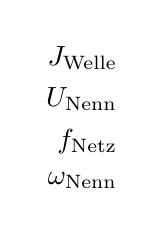
\begin{tikzpicture}[node distance=.5cm]
    \begin{scope}[]
    	    \matrix[column 1/.style={anchor=base east}]{
             \node[] {$J_{\mathrm{Welle}}$}; \\
             \node[] {$U_{\mathrm{Nenn}}$}; \\
             \node[] {$f_{\mathrm{Netz}}$}; \\
             \node[] {$\omega_{\mathrm{Nenn}}$}; \\
        };
    \end{scope}
\end{tikzpicture}
\end{document}